\documentclass[12pt]{article}
\usepackage[slovene]{babel}
\usepackage[utf8]{inputenc}
\usepackage[T2A]{fontenc}
\usepackage{amsmath}
\usepackage{amsfonts}
\usepackage{amssymb}
\usepackage[version=4]{mhchem}
\usepackage{stmaryrd}
\usepackage{graphicx}
\usepackage[export]{adjustbox}
\graphicspath{ {./images/} }
\usepackage{physics}
\usepackage{geometry}
\geometry{left=2cm,right=2cm,top=2cm,bottom=2cm}



\title{\textbf{Sklopljena nihajna kroga}}
\author{Samo Krejan}
\date{maj 2025}

\begin{document}
\maketitle

\section{Uvod}

Zelo pogosto se v naravi srečamo s pojavi, kjer gre za dva ali več nihal, ki so med seboj sklopljena. Zaradi omenjene sklopitvije nihal ne moremo več obravnavati ločeno temveč kot en sistem.

Sistem $n$ enakih in enostavnih oscilatorjev ima $n$ lastnih nihanj. V prvem letniku smo že spoznali obnašanje dveh sklopljenih fizičnih nihal; tam sta lastni frekvenci ko nihali nihata točno v fazi in ko nihata iz faze. Prva lastna frekvenca je kar enaka lastni frekvenci posameznega nihala, druga pa je hitrejša, če je sklopitev močnejša.

Pri tej vaji smo opazovali električna nihajna kroga sklopljena s kondenzatorjem. En sam nihajni krog sestavljen iz kondenzatorja s kapaciteto $C$ in tuljave z induktivnostjo $L$ niha s krožno frekvenco; 

$$\omega_0 = \frac{1}{\sqrt{LC}}$$

Če je v nihajnem krogu prisoten še upor $R$, nastopi dušenje, ki ga opišemo s koeficientom $\beta = R/2L$. Sistem opisujejo enačbe za dušeno nihanje z rešitvijo;

$$I(t) = e^{-\beta t} \left(I_1\sin{\omega ' t} + I_2\cos{\omega ' t}\right)$$

Kjer je $\omega ' = \sqrt{\omega_0^2 - \beta^2}$

Če k prvemu krogu vežemo še drugi preko kondenzatorja $C_0$ potem dobimo sklopljen sistem nihajnih krogov. zaradi dveh prostorskih stopenj imamo torej dva lastna načina nihanja; prvi je enak kot prej, ko oba nihata v fazi, drugi lasten način pa je:

$$U_{1,2} = \pm U_0 e^{-\beta t} \cos (\omega '' t)$$

kjer je $\omega '' = \sqrt{\frac{C}{C-C_0}\omega_0^2 - \beta^2}$.

Splošno obnašanje sistema lahko opišemo kot linearno kombinacijo obeh lastnih nihanj:

$$U_{1,2} = e^{-\beta t} \left(U' \cos (\omega' t) \pm U'' \cos (\omega '' t + \delta)\right)$$



\section{Potrebščine}

\begin{itemize}
\item Digitalni osciloskop,
\item funkcijski generator napetosti, namizni multimeter,
\item nihajna kroga in kabli, USB ključek,
\item prenosnik z ustrezno programsko opremo.
\end{itemize}


\section{Naloga}

\begin{enumerate}
\item Izmerite časovni potek napetosti na obeh krogih pri vzbujanju s stopničastim signalom za vse različne sklopitve,
\item Izmerite frekvenčno karakteristiko enega nihajnega kroga in določite dobroto $Q$
\item Izmerite frekvenčo karakteristiko sklopljenih nihajnih krogov z meritvijo odziva drugega kroga za vsak $C_0$ in izmerite razliko lastnih krožnih frekvenc
\end{enumerate}


\section{Rezultati in analiza}

Nihajna kroga sta sestavljena iz tuljave z induktivnostjo $L$, kondenzatorja s kapacitivnostjo $C = 5.6\ nF$ in uporom z upornostjo $R = 7.5\ \Omega$. Najprej smo priklopili nihajna kroga na osciloskop in vir stopničaste napetosti (glej sliko vezja). Izmerili smo odziv prvega in drugega kondenzatorja pri vseh različnih sklopitvah.

\begin{figure}[ht]
\begin{center}
    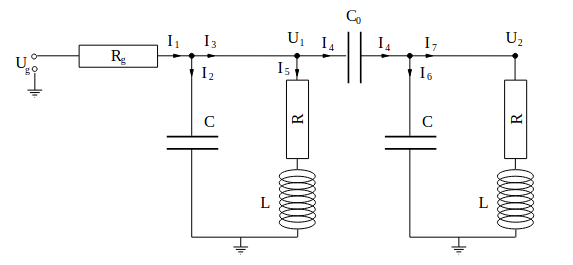
\includegraphics[width=10cm]{vezje.png}
    \caption{Skica vezja uporabljenega pri eksperimentu}
\end{center}
\end{figure}

Najprej smo merili odziv brez sklopitve $C_0 = 0$, a se je že tu izkazalo, da je prišlo do nekaj sklopitve. Tako smo že tu na grafa $U_1, U_2$ že na tej točki *fitali* funkciji:

$$U_1(t) = U_0 e^{-\beta t} \sin \left(\frac{\omega ' + \omega''}{2}t\right)\cos\left((\omega'-\omega'')t\right)$$

$$U_2(t) = U_0 e^{-\beta t} \sin \left(\frac{\omega ' + \omega''}{2}t\right)\sin\left((\omega'-\omega'')t\right)$$

Če bi na grafe risali tudi fite funkcij bi nastal kaos, tako da smo poleg izmerjenih podatkov risali zgolj ovojnico. Na ta način smo dobili naslednja grafa:
\newpage

\begin{figure}[h]
\centering
\begin{minipage}[t]{0.45\textwidth}
    \includegraphics[width=\textwidth]{p1.pdf}

\end{minipage}
\hfill
\begin{minipage}[t]{0.45\textwidth}
    \includegraphics[width=\textwidth]{p2.pdf}

\end{minipage}
\caption{$U_1, U_2$ izmerjena, ter njuni ovojnici pri minimalni sklopitvi}
\end{figure}

Iz fita dobimo vrednosti parametra $\omega' = 4.2\cdot 10^5 \ 1/s$, napake fita pa tu ne bom navajal, saj je manjša od procenta. Če predpostavimo $\omega >> \beta$ (kar lahko naredimo saj mo daleč od kritičnega dušenja), dobimo $L = 9.9\cdot 10^{-4} H$ Za tem smo praktično isti postopek ponovili še za ostale sklopitve. Primer meritve in ovojnice fita vidimo na naslednjih dveh grafih:

\begin{figure}[h]
\centering
\begin{minipage}[t]{0.45\textwidth}
    \includegraphics[width=\textwidth]{p3.pdf}

\end{minipage}
\hfill
\begin{minipage}[t]{0.45\textwidth}
    \includegraphics[width=\textwidth]{p4.pdf}

\end{minipage}
\caption{$U_1, U_2$ izmerjena, ter njuni ovojnici pri minimalni sklopitvi}
\end{figure}
Ko smo tako fitali omenjeno funkcijo na podatke smo dobili naslednje vrednosti predstavljene v tabeli:

\begin{table}[!ht]
\centering
\begin{tabular}{c|c|c|c}
    $C$ [$pF$] & krog & $\beta$ [$s^{-1}$] & $\Delta  \omega$ [$s^{-1}$] \\\hline \hline

    $330$ & $U_1$ & $6262 \pm 2$ & $18996 \pm 2$\\
    & $U_2$ & $6585\pm 2$ & $18887 \pm 1$\\
    $560$ & $U_1$ & $6080\pm 2$ & $26368\pm 2$\\
    & $U_2$ & $6347\pm 2$ & $26302\pm 1$\\
    $820$ & $U_1$ & $5976\pm 2$ & $33644\pm 2$\\
    & $U_2$ & $6200\pm 2$ & $33600\pm 1$\\
    $1150$ &$U_1$ & $6252\pm 1$ & $40368\pm 1$\\
    & $U_2$ & $6430\pm 2$ & $40338\pm 1$\\\hline \hline
    povprečje && $6300\pm 300$ &
\end{tabular}
\caption{Tabela izmerjenih vrednosti}
\end{table}
kjer je $\Delta \omega = \omega' - \omega''$. Če $\beta$ izračunamo iz podanega upora in prej izračunane induktivnosti dobimo:

$$
\beta' = \frac{R}{2L} = 3787\ s^{-1}
$$
kar zelo močno odstopa od izmerjene vrednosti. Razlog za to je v morda večjem uporu, ali kakšni drugi neidealizaciji. Frekvence utripanja smo nato nanesli na graf v odvsnosti od sklopitvenega kondenzatorja:

\begin{figure}[ht]
\begin{center}
    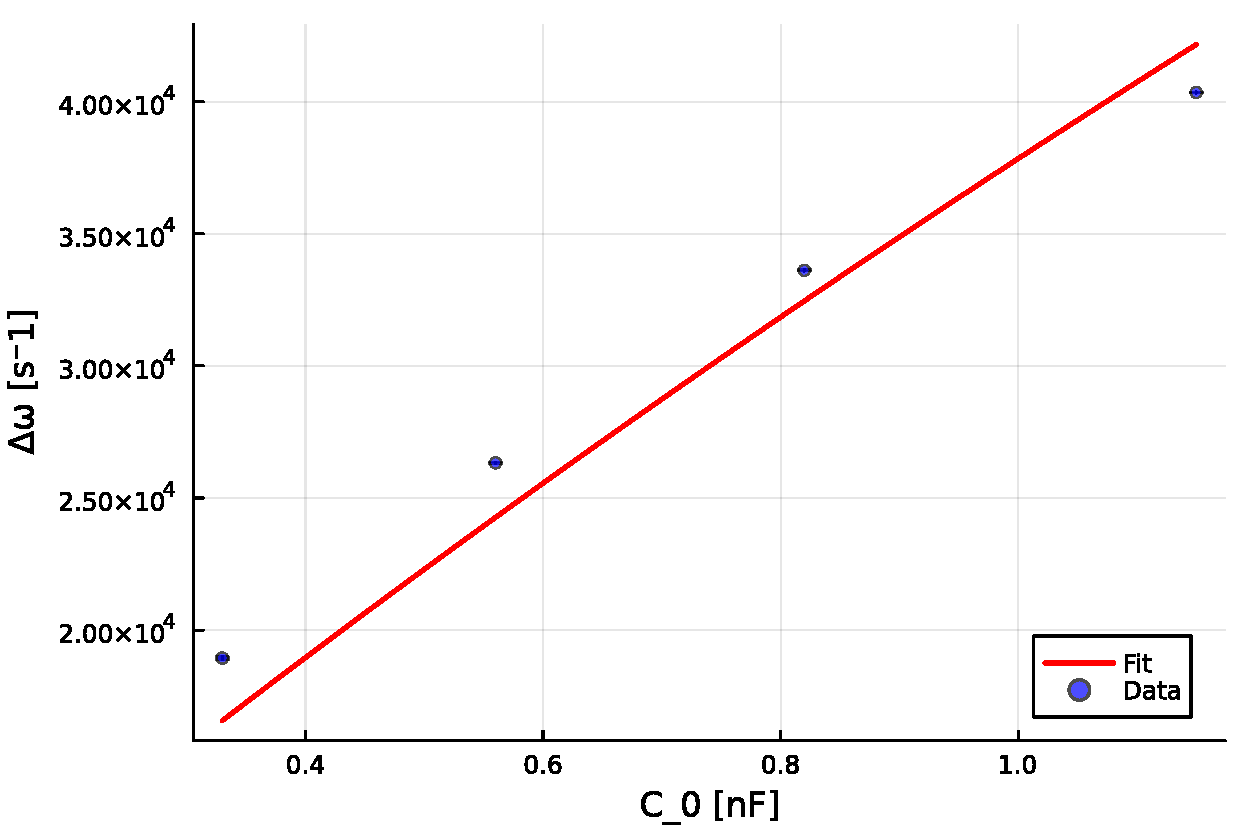
\includegraphics[width=10cm]{freq.pdf}
    \caption{Frekvenca utripanja v odvisnosti od sklopitvenega kondenzatorja s fitom}
\end{center}
\end{figure}
Na grafu je poleg meritev tudi fit, ki smo ga dobili s teoretično funkcijo:

$$
\Delta \omega = \omega' - \omega '' + (\omega)_I
$$
kjer je $\omega'$ izmerjena z veliko natančnostjo, $\omega ''$ izračunana iz sklopitvenega kondenzatorja, kot je opisano v uvodu in $(\omega)_I$ je parameter, ki verjetno pride zaradi induktivnosti sklopitve. Glede na fit znaša $(\omega)_I = (5000 \pm 1000)\ s^{-1}$

Za tem smo opazovali resonančni odziv na vsiljeno nihanje brez sklopitvenega kondenzatorja. Merili smo na dva načina; ko je bil drugi krog prizemljen, in ko je bil neprizemljen. Ko je bil drugi krog neprizemljen vidimo dva vrhova, ki ustrezata dvema različnima nihajnima načinoma. Tega načeloma ne bi smeli opaziti, saj nismo imeli nobene sklopitve, a to vseeno lahko razložimo, z neko induktivno sklopitvijo, kot smo to storili tudi v prejšnjem delu vaje.

\begin{figure}[ht]
\begin{center}
    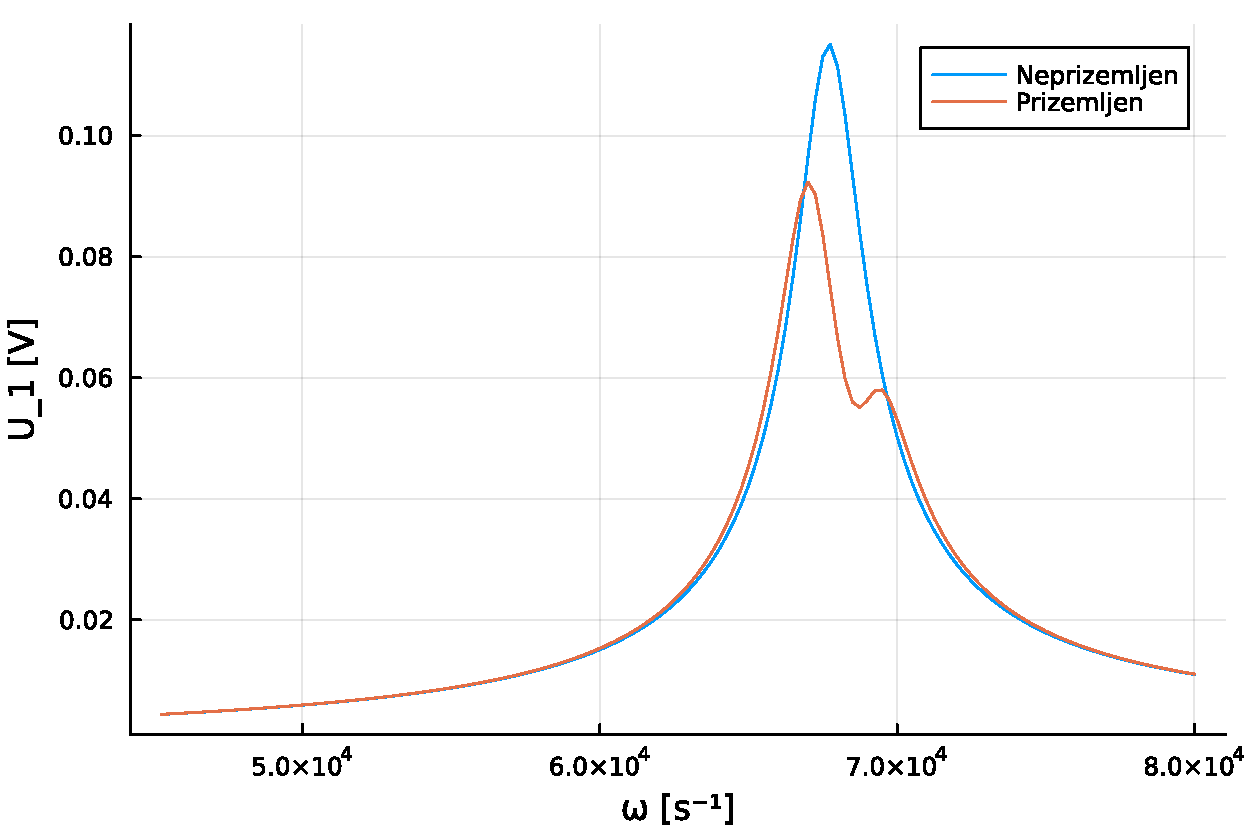
\includegraphics[width=10cm]{odziv.pdf}
    \caption{resonančni odziv nesklopljenih nihal, ko je drugo (ne)ozemljeno}
\end{center}
\end{figure}
Če se osredotočimo samo na graf neprizemljenega drugega kroga, lahko določimo dobroto $Q$ prvega nihajnega kroga. Ta je definirana kot $Q = \frac{\omega_0}{\Delta \omega}$, kjer je $\omega_0$ resonančna frekvenca in $\Delta \omega$ širina resonančne krivulje. Na ta način dobimo:

$$
Q = 33.8 \pm 8.5
$$

\newpage
Za tem smo nadaljevali z drugim nihajnim krogom prizemljenim, in opazovali odziv. Pri vsaki meritve smo dobili dva maksimuma, kjer je vsak predstavljal eno izmed lastnih nihanj sistema. Opazimo, da je en stalno na istem mestu, to je nihanje ki je ekvivalentno nihanju enega samega nihajnega kroga in ni odvisno od sklopitve, medtem ko drugo je odvisno od sklopitve. Zanima nas odvisnost razlike teh maksimumov od sklopitve.

\begin{figure}[ht]
\begin{center}
    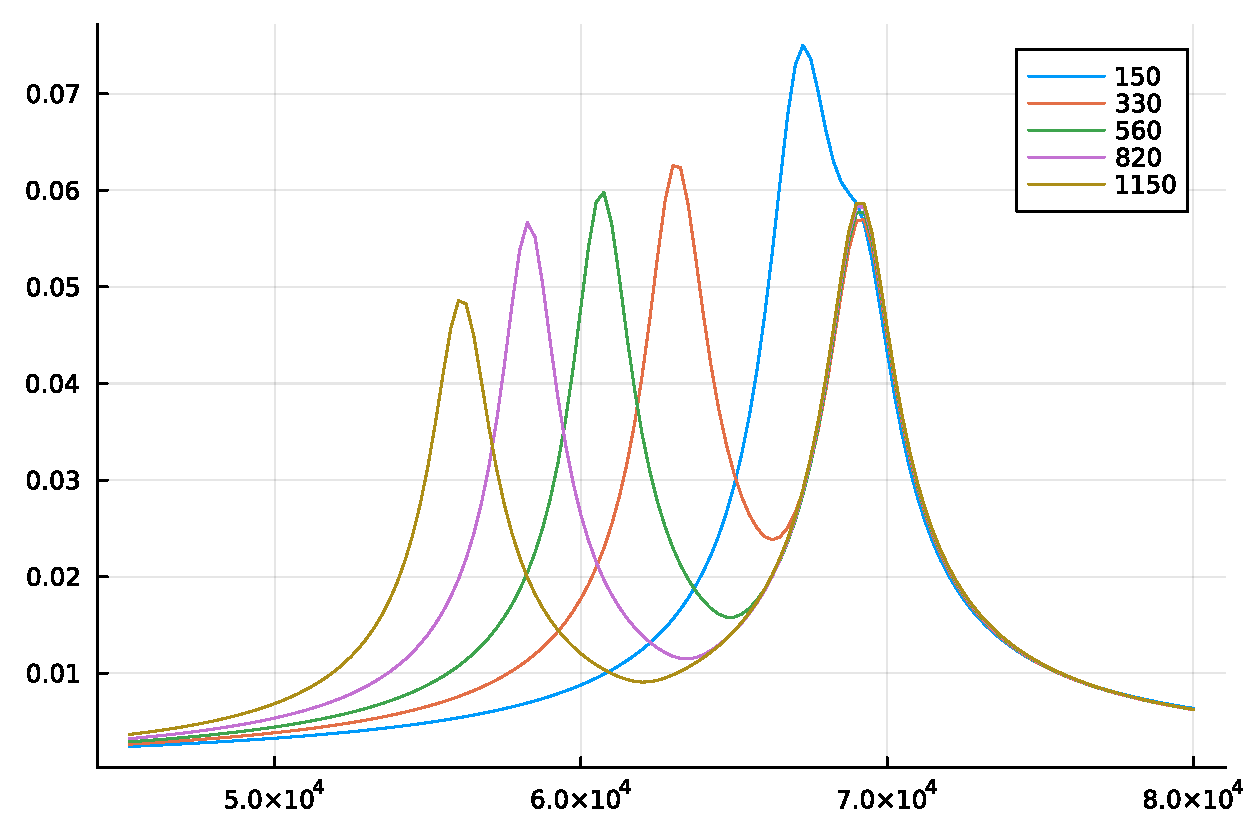
\includegraphics[width=10cm]{multi.pdf}
    \caption{Resonančni odziv sklopljenih krogov pri drugačnih sklopitvah}
\end{center}
\end{figure}


\end{document}